\section{Question 3: Fixed-split cross-GPU substitution}
\label{sec:r2q3}
\subsection{Model and two route rules}
A job has native model $n_j$, actual model $m_j$, duration $p_j$, workers $W_j$, and per-worker requests $(g_j,c_j)$. For the sole assumed foreign edge A10$\to$A100-SXM4-80GB, $p'_j=\sigma p_j$; compatibility and $\sigma$ are scenario assumptions, not measured hardware facts. All workers start together on physical nodes, with no migration or preemption, and every start passes the same CPU/GPU slot check.

The no-substitution baseline keeps each job in its native pool. The Hash-10\% rule reserves 60 of 432 A100 nodes for a deterministic 10\% selected A10 subset. The implemented Shape-filtered rule keeps only selected jobs whose CPU/GPU shape fits the donor ratio, yielding 10,604 routed and 605 shape-rejected A10 jobs. It is a fixed physical counterfactual, not a claim that a dynamic policy has been implemented. Source mappings for the main and sensitivity scenarios are in the supplement.

\begin{table}[H]\centering
\caption{Fixed-split results: (a) performance. Waiting and JCT use complete drain; completions use the 90-day horizon.}
\label{tab:q3main}
\begin{tabular}{lrrrrr}
\toprule
Scenario & $\sigma$ & \shortstack{A10 mean\\wait (h)} & \shortstack{A10 mean\\JCT (h)} & \shortstack{All mean\\JCT (h)} & \shortstack{90-day\\completions}\\
\midrule
No substitution & --- & 32.906 & 132.676 & 93.334 & 217,578\\
Hash-10\% & 1 & 20.534 & 120.303 & 87.190 & 217,822\\
Hash-10\% & 2 & 25.106 & 134.810 & 94.393 & 217,529\\
Shape-filtered & 1 & 24.359 & 124.128 & 89.089 & 217,809\\
Shape-filtered & 2 & 24.359 & 129.671 & 91.842 & 217,621\\
\bottomrule
\end{tabular}

\end{table}
\addtocounter{table}{-1}
\begin{table}[H]\centering
\caption{Fixed-split results: (b) harm relative to the No-substitution baseline. A10 harm means a later completion; native A100 harm means increased waiting.}
\label{tab:q3harm}
\begin{tabular}{lrrr}
\toprule
Scenario & $\sigma$ & \shortstack{Native A100\\increased-wait jobs} & \shortstack{A10 later-\\completion jobs}\\
\midrule
No substitution & --- & 0 & 0\\
Hash-10\% & 1 & 0 & 49,772\\
Hash-10\% & 2 & 0 & 56,422\\
Shape-filtered & 1 & 0 & 46,803\\
Shape-filtered & 2 & 0 & 55,465\\
\bottomrule
\end{tabular}
\smallskip\par Both parts use SPT-HOL, GS1 ratio placement, and FF-id in the other pools. Substitution scenarios dedicate 60 A100 nodes to foreign jobs. No substitution keeps the full native pools and has no foreign partition.
\end{table}


\WinnerClaim{} The per-scenario FCFS A10 means are 687.645 versus 756.125 h at $\sigma=1$ and 831.456 versus 761.668 h at $\sigma=2$; for SPT-HOL they are 120.303 versus 124.128 h and 134.810 versus 129.671 h, respectively (Hash-10\% versus Shape-filtered). Thus the two-point maxima are 831.456 versus 761.668 h for FCFS and 134.810 versus 129.671 h for SPT-HOL. These are evaluated points, not an upper bound over an interval, an unknown-speed guarantee, or a unique $\sigma^*$.

\subsection{What the trade-off means}
For SPT-HOL, Hash-10\% is the more aggressive 10\% split; Shape-filtered rejects 605 high-CPU/GPU jobs and changes the selected load. At the tested $\sigma=1$ point, Hash-10\% reduces A10 wait relative to the No-substitution baseline, while Shape-filtered has a smaller A10 benefit but lower paired positive completion-delay mass (16,051.659 job-hours versus Hash-10\% at 68,183.183 job-hours). At $\sigma=2$, common routed-job ordering is unchanged because all durations in one foreign queue are multiplied by the same $\sigma$; re-simulation is still required because completion/release interactions change. Shape-filtered's A10 wait is unchanged at 24.359 h between the two evaluated speeds, but A10 JCT rises 5.542 h and 90-day completions fall by 188.

The A100 allocation uses two explicit denominators. Partition-own rates are computed within each partition: for Hash-10\%, native/foreign are 0.728770/0.682727 at $\sigma=1$ and 0.728770/0.669479 at $\sigma=2$; for Shape-filtered they are 0.728770/0.449232 and 0.728770/0.628414. The full-pool contributions are respectively 0.627552/0.094823, 0.627552/0.092983, 0.627552/0.062393, and 0.627552/0.087280, and each satisfies $U_{\rm all}=(2976U_{\rm native}+480U_{\rm foreign})/3456$, giving 0.722376, 0.720535, 0.689946, and 0.714832. Thus the Shape-filtered foreign partition is 44.923\% allocated and 55.077\% idle at $\sigma=1$, versus 62.841\% allocated and 37.159\% idle at $\sigma=2$; these are partition-own rates and are not full-pool contributions. A larger partition rate is not called a utilization gain by shrinking the native denominator.

The aggregate capacity conversion $534/8=66.75$ is only a pooled arithmetic quantity; it is not rounded to 67 nodes and is not a node-level safe-borrow certificate. The conclusion that 60 donor nodes produce zero native harm is supported by the formal physical schedule, while host safety still depends on node-level placement checks.

\begin{figure}[H]\centering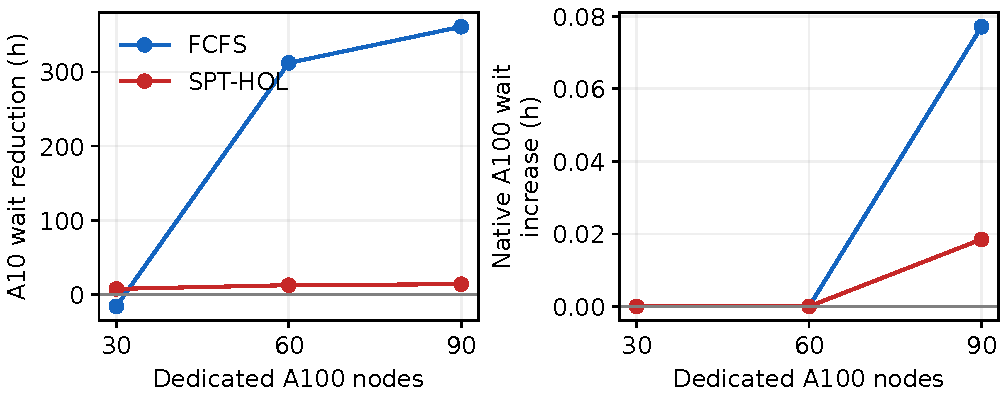
\includegraphics[width=\linewidth]{figures/q3_donor_capacity_wait_tradeoff.pdf}\caption{Donor-capacity sensitivity at 10\% routing and $\sigma=1$, relative to the No-substitution baseline. Left: A10 mean-wait reduction; right: native A100 mean-wait increase. The panels use separate scales.}
\label{fig:r2q3tradeoff}\end{figure}

The sensitivity analysis retains negative cases: at 60 donors, 20\% routing raises FCFS A10 mean wait to 1,010.136 h and its maximum to 5,445.367 h; 30 donors at 10\% gives 916.407 h, worse than No substitution. For the 90-donor case, SPT-HOL native A100 has 2,150 positive-delay jobs, mean additional wait 0.018492 h over all 80,877 native jobs, and harmed-subgroup mean 0.695606 h. These finite paired results expose the management choice between A10 relief, native harm, tail, and completion count.

A financial extension is optional rather than a second experiment. If a tenant values completion time at $v$ per hour and pays $P$, voluntary substitution requires payment reduction at least $v$ times the completion-time increase. No price, participation rate, revenue, or profitability is inferred here. An online completion-cost routing rule remains future work.
